\documentclass[10pt]{scrartcl}

\usepackage[utf8]{inputenc}
\usepackage{tabularx}
\usepackage[ngerman]{babel}
\usepackage[automark]{scrpage2}
\usepackage{amsmath,amssymb,amstext}
%\usepackage{mathtools}
\usepackage[]{color}
\usepackage[]{enumerate}
\usepackage{graphicx}
\usepackage{lastpage}
\usepackage[perpage,para,symbol*]{footmisc}
\usepackage{listings} 
\usepackage[pdfborder={0 0 0},colorlinks=false]{hyperref}
\usepackage[numbers,square]{natbib}
\usepackage{color}
\usepackage{colortbl}
\usepackage{listings}
\usepackage{a4wide}
\usepackage{xspace}
\usepackage{listings}
\usepackage{hyperref}
\usepackage{epstopdf}

\lstset{numbers=left, numberstyle=\tiny, numbersep=5pt, breaklines=true, showstringspaces=false} 

%changehere
\def\titletext{TH1 Praktikum 1 : Ausarbeitung}
\def\titletextshort{Praktikum 1}
\author{Carsten Noetzel, Armin Steudte}

\title{\titletext}

%changehere Datum der Übung
\date{23.03.2012}

\pagestyle{scrheadings}
%changehere
\ihead{TH1, Padberg}
\ifoot{Generiert am:\\ \today}

\cfoot{Carsten Noetzel, Armin Steudte}


\ohead[]{\titletextshort}
\ofoot[]{{\thepage} / \pageref{LastPage}}

\setlength{\parindent}{0.0in}
\setlength{\parskip}{0.1in}

\begin{document}
\maketitle

\setcounter{tocdepth}{3}
\tableofcontents
\listoffigures
%\lstlistoflistings

\section{Aufgabe 1 - Aufbau des Petrinetzes}

%\begin{figure}[htbp]
%	\centering	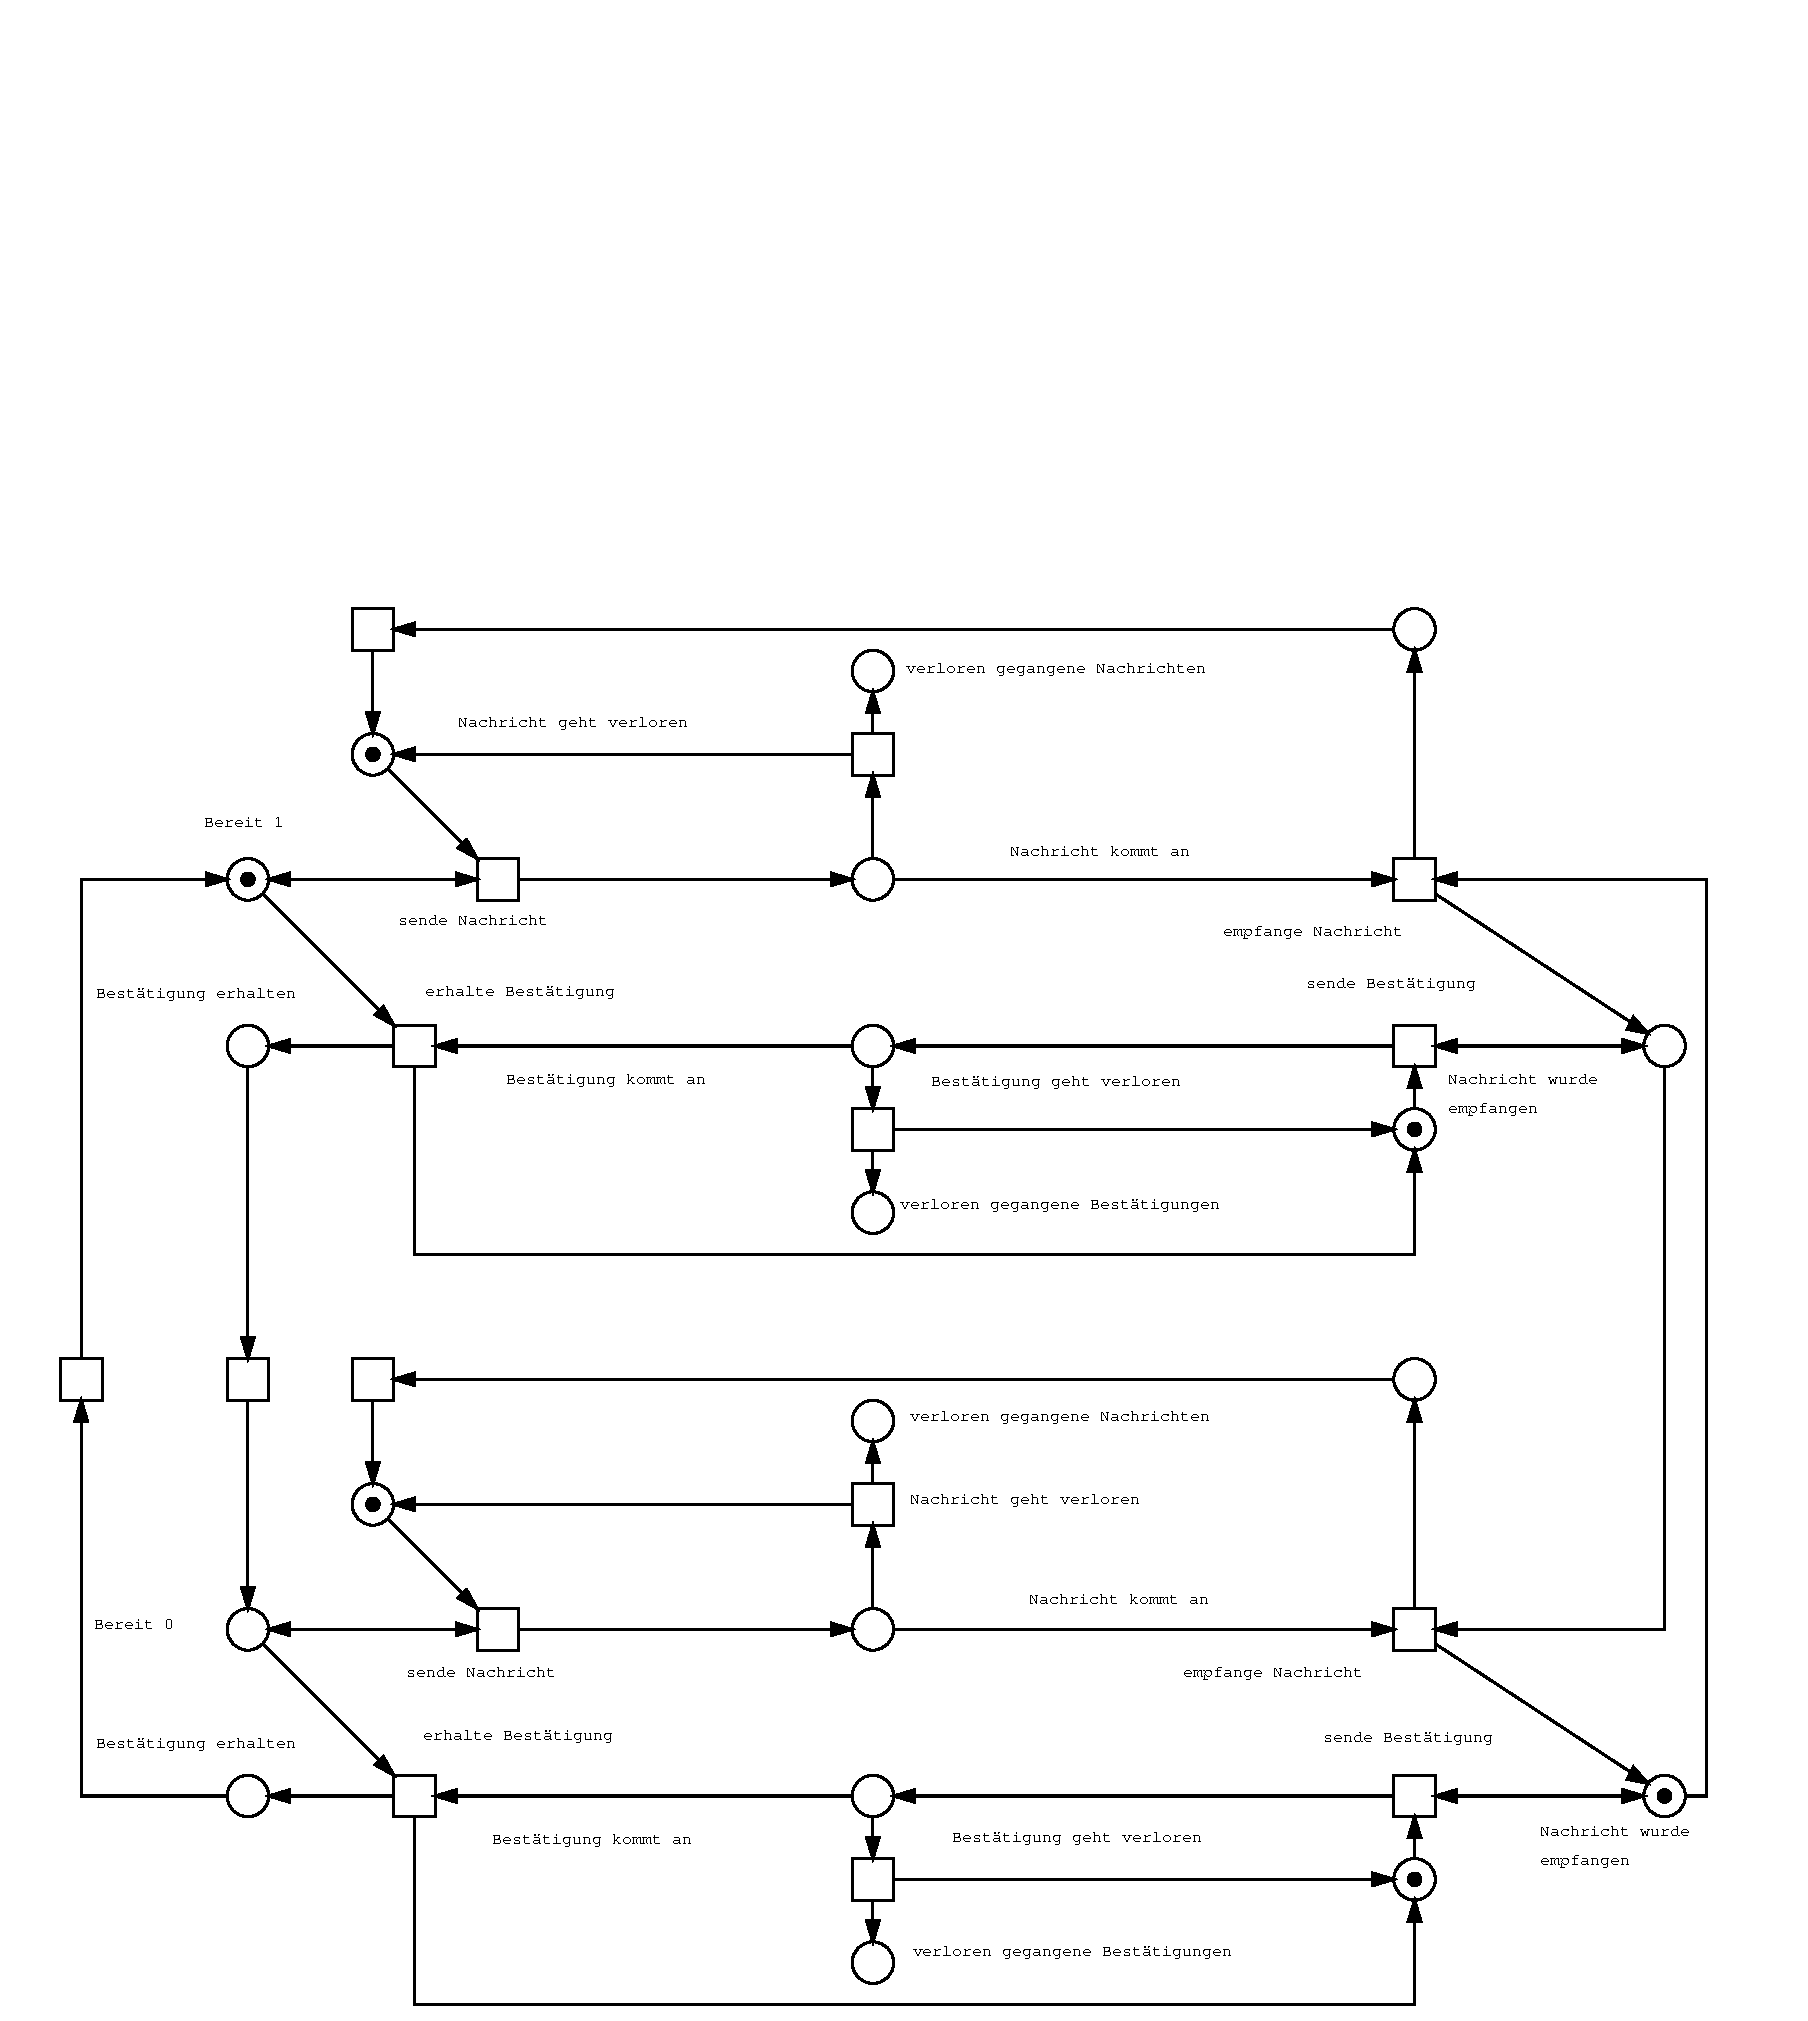
\includegraphics[width=1.0\textwidth]{Grafiken/Praktikum1_1.eps}
%	\caption{Petrinetz}
%	\label{fig:Netz}
%\end{figure} 

\section{Aufgabe 2 - Erläuterungen zur Modellierung}

\section{Aufgabe 3 - Begründung der Korrektheit}

\section{Aufgabe 4 - Nachrichtenverlust}

\section{Aufgabe 5 \& 6 - Erweiterung des Systems}
\subsection{Von 20 Nachrichten maximal 1 Nachricht Verlust}
\label{sec:nachrichtenverlust_1}
Um die in der Aufgabe gestellte Anforderung, nicht mehr als eine Nachricht von 20 gesendeten zu verlieren, erfüllen zu können, müssen alle vier Sendeprozesse (Nachrichtenversand mit Bit 1, Nachrichtenversand mit Bit 0, Empfangsbestätigung mit Bit 1 und Empfangsbestätigung mit Bit 0) angepasst werden.\\
Beispielhaft ist in Abbildung \ref{fig:Erweiterung5} die Erweiterung des Prozesses, zum Versand der Nachricht mit Korrekturbit 1, abgebildet.
Ausgehend von der Transition "`empfange Nachricht"' wurde über einer Stelle ein Zähler für die Anzahl empfangener Nachrichten realisiert. 
Die Idee dahinter war es einen Schaltmechanismus zu realisieren, der dafür sorgt, dass sobald eine Nachricht verloren gegangen ist, die nächsten 19 Nachrichten empfangen werden.\\
Zu diesem Zweck wurde die Transition "`Nachricht geht verloren"' um eine weitere Vorbedingung ergänzt, die die Transition nur schalten lässt wenn nach der ersten verlorenen Nachrichten erfolgreich empfangen wurden. Die Stelle die dabei als Vorbedingung fungiert besitzt zum Anfang ein Token (eine Nachricht kann damit zu Anfang verloren gehen).
Diese Stelle wurde über eine Transition mit dem Zähler für die empfangenen Nachrichten verbunden.
Die Kante von der Stelle, zum Zählen der empfangenen Nachrichten, hin zur Transition wurde mit einem Gewicht von 19 versehen.
Dieses stellt sicher, dass sobald eine Nachricht verloren gegangen ist, die nächsten 19 empfangen werden.  

\begin{figure}[htbp]
	\centering	\includegraphics[width=1.0\textwidth]{Bilder/Erweiterung_Aufgabe_5}
	\caption{Erweiterung Aufgabe 5}
	\label{fig:Erweiterung5}
\end{figure}

\subsection{Pro gesendeter Nachricht maximal 20 Nachrichten Verlust}
Bei dieser Teilaufgabe wurde ein ähnlicher Ansatz wie in der Vorangegangenen gewählt.
Um die Anforderung realisieren zu können muss die Stelle, die vorher als Schalter agierte, nun die Funktion eins Token Buckets übernehmen.
Das Ziel ist es mit jeder empfangener Nachricht zusätzlich 20 neue Tokens in den Eimer zu tun.
Beim Verlust einer Nachricht wird gleichzeitig ein Token aus dem Eimer konsumiert, so dass Nachrichten nur verloren gehen können wenn der Eimer Tokens enthält.
Das Konstrukt stellt so die Obergrenze von 20 verlorenen Nachrichten sicher.
Der Nichtdeterminismus bestimmt dabei immer noch ob eine Nachricht verloren geht oder empfangen wird.
Diese Mechanismus wird auch bei allen Sendeprozesse realisiert.\\
Im Petrinetz muss hierzu die Lösung aus Abschnitt \ref{sec:nachrichtenverlust_1} mit kleinen Modifikationen versehen werden.
Das Kantengewicht der Vorbedingung der Transition von 19 wird auf 1 gesetzt und die Nachbedingung, also das Kantengewicht der Kante von der Transition zur Stelle die den Eimer darstellt, wird auf 20 gesetzt.
So werden jedes Mal wenn ein Token den Empfänger erreicht 20 neue Tokens in den Token Bucket getan, welches den Verlust von Nachrichten auf 20 pro empfangener Nachricht limitiert. 
 
\begin{figure}[htbp]
	\centering	\includegraphics[width=1.0\textwidth]{Bilder/Erweiterung_Aufgabe_6}
	\caption{Erweiterung Aufgabe 6}
	\label{fig:Erweiterung6}
\end{figure}

\end{document}

